% !TEX root = ../Masterarbeit.tex
\chapter{Hauptteil}

\section{Design Patterns}
Viele der angesprochenen Probleme oder Lösungsansätze sind nicht neu. Programme wartbar und erweiterbar zu gestalten ist ebenfalls keine neue Anforderung. Beispielsweise ist der Ansatz, Komponenten voneinander zu entkoppeln seit Langem ein Ziel bei der Entwicklung von Software.\\
Die meisten Probleme sind wiederkehrende Probleme, die bereits schon einmal gelöst wurden. Ein Design Pattern (dt. Entwurfsmuster) ist eine Vorlage zur Lösung eines wiederkehrenden Problems. Der Architekt Christopher Alexander prägte den Begriff Design Pattern durch sein Buch \enquote{A Pattern Language}, in dem er eine allgemeingültige Sprache für wiederkehrende Probleme der Architektur definiert.\\
Zu Beginn des Buches beschreibt er die Sprache wie folgt~\cite[S. \textit{x}]{alexander_pattern_1977}:

\begin{quotation}
The elements of this language are entities called patterns. Each pattern describes a problem which occurs over and over again in our environment, and then describes the core of the solution to that problem, in such a way that you can use this solution a million times over, without ever doing it the same way twice.
\end{quotation}

Diese Definition haben Gamma et al in ihrem Buch \enquote{Design Patterns} aufgegriffen und auf die Entwicklung objektorientierter Software übertragen. Ein Design Pattern bietet keine fertige Lösung sondern einen Lösungsansatz für generalisierte Probleme. Die Abstraktion von Problemen durch Design Patterns kann auf unterschiedlichen Ebenen erfolgen. Design Patterns können die Struktur bzw. Architektur von Systemen, deren Komponenten oder auch im Detail die Klassen beeinflussen~\cite[S.~3]{gamma_design_1995}~\cite[S.~127]{douglass_real-time_2003}. Deshalb können Patterns klassifiziert und gruppiert werden. Es gibt beispielsweise Architektur- oder Verhaltensmuster.\\
Ein Pattern beschreibt, ein generalisiertes Problem sowie einen entsprechenden allgemeinen Lösungsansatz. Durch die Definition von Design Patterns wird eine gemeinsame und allgemeingültige Sprache für die Probleme der Software Entwicklung geschaffen.\\
Ein Pattern besteht grundsätzlich aus vier Teilen~\cite[S.~3]{gamma_design_1995}:

\begin{enumerate}
\item Einem sprechenden und eindeutigen \textbf{Namen}, welcher das Problem und die Lösung in nicht mehr als zwei oder drei Wörtern beschreibt.
\item Eine Beschreibung des \textbf{Problems}, welches das Pattern zu lösen vermag. Wichtig ist hierbei auch der Kontext bzw. die Sichtweise auf das Problem.
\item Die eigentliche \textbf{Lösung} des Problems in Form von Diagrammen und Beschreibung. Die Lösung sollte jedoch allgemeingültig und technologieunabhängig sein.
\item Zudem sollten die \textbf{Konsequenzen} --- also Vor- und Nachteile, die durch die Verwendung des Pattern entstehen, genannt werden.
\end{enumerate}

Reaktives Software Design schließt von vornherein bereits einige Patterns aus --- vor allem bedingt durch die lose Kopplung sowie die asynchrone und nachrichtenorientierte Kommunikation zwischen den Komponenten. Als Folge dessen entstehen jedoch neue Problemfelder. Die Vergangenheit hat gezeigt, wie hilfreich Design Patterns bei der Lösung von Problemen sein können. Deshalb ist es nur sinnvoll sich mit Design Patterns zu beschäftigen, die ein reaktives Software Design im Sinne des Reactive Manifestos unterstützen~\cite[S.~54]{kuhn_reactive_2015}.

\pagebreak

\section{Concurrency Modelle}
Die Basis eines reaktiven Systems, ist das zugrundeliegende Concurrency Modell. Ein reaktives System besteht aus vielen isolierten Komponenten, die asynchron miteinander kommunizieren. Diese Komponenten können in einem Computercluster verteilt sein und arbeiten zudem weitestgehend unabhängig von einander und parallel. Die Programmierung von stark nebenläufigen Anwendungen durch systemnahe Konzepte, wie Threads und Locks ist kompliziert und fehleranfällig~\cite[S.~72]{erb_concurrent_2012}.\\
Im diesem Kapitel werden zwei Concurrency Modelle erklärt, die die Komplexität nebenläufiger Anwendungen isolieren und abstrahieren. Die Concurrency Modelle \enquote{Reactor Pattern} und \enquote{Actor Modell} arbeiten asynchron und nicht blockierend. Um deren Funktionalität aufrecht zu erhalten, ist es erforderlich, dass das darauf aufbauende System ebenfalls asynchron und nicht blockierend arbeitet~\cite[S.~171]{kuhn_reactive_2015}.

\subsubsection{Asynchrone Datenübertragung}\label{subsec:async-io}
Im vorangegangen Kapitel wurde erläutert, dass die Kommunikaktion zwischen den Komponenten asynchron erfolgen muss (siehe \autoref{subsec:communication}). Jedoch ist traditionellerweise der schreibende und lesende Zugriff auf Ressourcen, wie Netzwerk oder Festplatte synchron und blockierend. Das bedeutet, die Anwendung bzw. der Thread, ist für die gesamte Dauer des Zugriffs ausschließlich mit beispielsweise dem Abspeichern einer großen Datei beschäftigt.\\
\textit{Asynchronous I/O} ist ein Mechanismus moderner Betriebsysteme, welcher den asynchronen und nicht blockierenden Zugriff auf Ressourcen, wie Netzwerk, Arbeitsspeicher oder Festplatte ermöglicht.

\pagebreak

Folgende Abbildung (\ref{fig:async-io}) zeigt einen typischen Ablauf einer asynchronen und nicht blockierenden Datenübertragung. Dieses Modell erlaubt Anwendungen die gleichzeitige Bearbeitung von Datenübertragungen und weiteren Berechnungen. 

\begin{figure}[H]
 \centering
 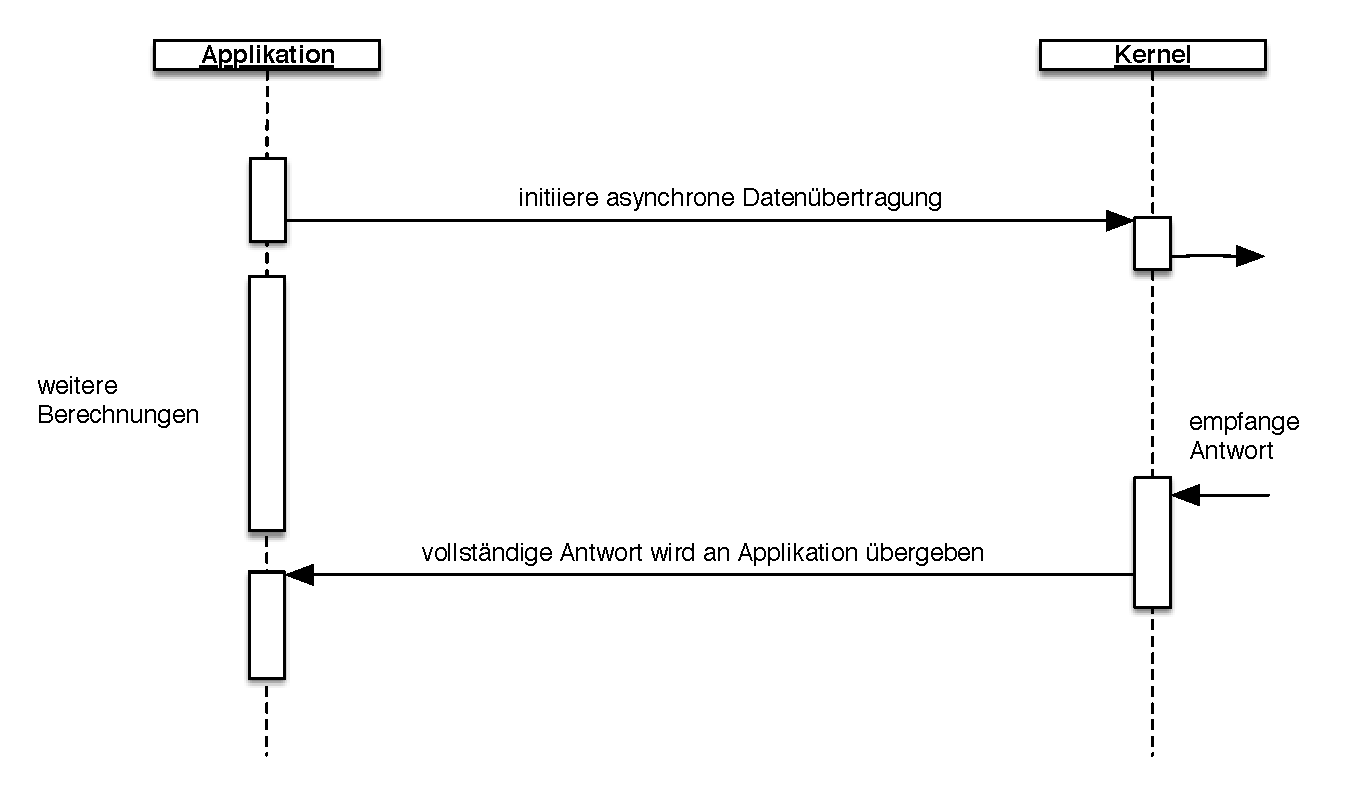
\includegraphics[width=1.0\textwidth]{4-Hauptteil/async-io/async-io.eps}
 \caption{Ablauf einer asynchronen und nicht blockierenden Datenübertragung}
 \label{fig:async-io}
\end{figure}

Die Anwendung kann nach der Initiierung der Datenübertragung sofort mit weiteren Berechnungen fortfahren. Das Betriebssystem informiert die Anwendung über die erfolgreiche Übertragung und übergibt die vollständige Antwort an die Anwendung. Durch diesen Mechanismus ist es möglich mit einem Thread mehrere Datenübertragungen asynchron abzuarbeiten, da diese den Thread nicht, wie traditionellerweise blockieren~\cite{jones_boost_2006}.

\pagebreak

Eine Webapplikation ist meist stark an Datenübertragung gebunden. Sei es die eigentliche HTTP Schnittstelle, der Zugriff auf die Datenbank oder die Kommunikation mit anderen Services. Eine Anfrage hat meist zur Folge, dass auf eine Datenbank zugegriffen wird. Die Ergebnisse der Datenbankanfrage werden aufbereitet und an den Client zurückgegeben. Der eigentliche Aufwand für die CPU ist relativ gesehen sehr gering.\\
Eine traditionelle Multi-threaded Webapplikation weist jeder eingehenden Anfrage einen dediziert Thread zu. Mit synchroner und blockierender Datenübertragung ist dieser Thread so lange blockiert bis die Antwort auf die Anfrage beim Client eingegangen ist. Ein Client mit einer langsamen Netzwerkanbindung blockiert deshalb einen Thread länger, wie ein Client mit einer schnellen Netzwerkanbindung.\\
Um eine Multi-threaded Webapplikation skalieren zu können, setzt man Thread pools ein, die eine vielzahl von Threads vorhalten --- meist weit aus mehr als der Prozessor Kerne hat. Jedoch ist die Koordination der Threads aufwendig und hat häufiges \textit{context switching} zur Folge.\\
Mit dem Modell der asynchronen und nicht blockierenden Datenübertragungen lassen sich Ressourcen effizienter nutzen. Zudem erhält man eine bessere vertikale Skalierung, als beispielsweise beim beschriebenen \enquote{One thread per request} Modell~\cite[S.~171]{butcher_seven_2014}~\cite[S.~76]{erb_concurrent_2012}.

\pagebreak

\subsection{Ereignisbasierte Concurrency}\label{subsec:eventdriven-concurrency}
Viele Anwendungen nutzen das Konzept der Events, um den Ablauf der Ausführung zu steuern. Man spricht auch von ereignisorientierter Software.\\ 
Ein Event ist ein Ereignis respektive ein Signal über eine Zustandsänderung. Im Gegensatz zu einer Nachricht hat ein Event keinen expliziten Empfänger, also keine Zieladresse. Komponenten können sogenannte Event handler an einem System registrieren. Diese werden dann über Zustandsänderungen informiert bzw. aufgerufen. Solange es zu keiner Zustandsänderung kommt, wird auch kein Event handler aufgefordert, ein Event zu verarbeiten. Die Komponente bleibt somit inaktiv~\cite[S.~91]{erb_concurrent_2012}.

\subsubsection{Reactor Pattern}
Ereignisorientierte Anwendungen müssen in der Regel viele Events von vielen verschiedenen Quellen koordinieren und abarbeiten. Beispielsweise ist jede Anfrage an eine Webanwendung ein Event und jeder Client folglich eine Quelle. Die Anfragen bzw. die Events können auch parallel bei der Anwendung eintreffen.\\
Um die Events abzuarbeiten, wird oft auf das Reactor Pattern zurückgegriffen (\autoref{fig:event-loop}). Events aus verschiedensten Quellen werden serialisiert und Event für Event abgearbeitet bzw. an die entsprechenden Event handler übergeben. Die Ausführung der Event handler erfolgt synchron. Die Reactor Komponente arbeitet in einer Endlosschleife, genannt Event loop~\cite[S.~260~-~S.~261]{buschmann_pattern_2011}.

\begin{figure}[H]
 \centering
 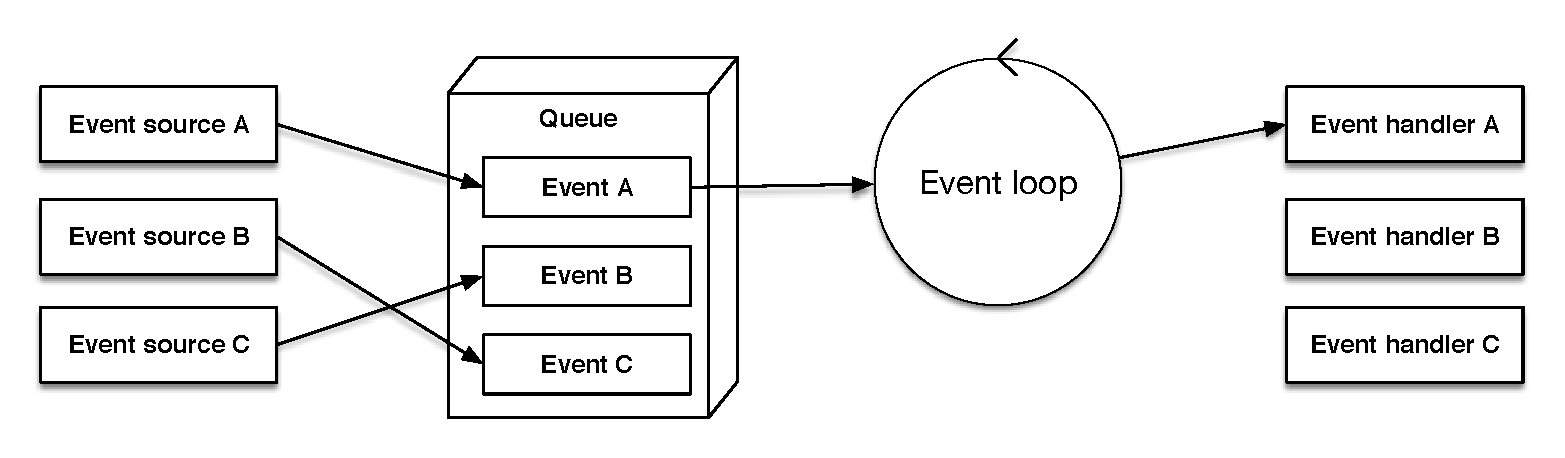
\includegraphics[width=1.0\textwidth]{4-Hauptteil/event-loop/event-loop.eps}
 \caption{Graphische Darstellung der Funktionsweise des Reactor Patterns}
 \label{fig:event-loop}
\end{figure}

Die Event loop wird typischerweise von genau einem Thread ausgeführt. Um dennoch nebenläufig mehrere Anfragen verarbeiten zu können, nutzt man Asynchronous I/O (siehe \autoref{subsec:async-io}). So ist es möglich nebenläufig, mit nur einem Thread, auf Events von vielen verschiedenen Quellen zu reagieren. Ein Event handler blockiert während der synchronen Ausführung, die Event loop und somit die Abarbeitung weiterer Events. Folglich ist das Reactor basierte Concurrency Modell nur für datenübertragungsintensive Applikationen, die von Asynchronous I/O profitieren, sinnvoll~\cite[S.~73]{kuhn_reactive_2015}~\cite[S.~92]{erb_concurrent_2012}.\\
Mit dem Reactor Pattern ist es möglich viele Anfrage nebenläufig, mit nur einem Thread, zu verarbeiten. Es entsteht kein Performance Overhead, wie bei traditionellen \enquote{One thread per request} Applikationen. Zudem wird die Komplexität der nebenläufigen Verarbeitung in der Reactor Komponente gekapselt und der Entwickler muss nicht mit den typischen Problemen der nebenläufigen Programmierung kämpfen. Außerdem können Event handler leicht wiederverwendet und kombiniert werden.\\
Es gibt zwei populäre Implementierungen dieses Concurrency Modells. Zum einen das JavaScript (V8) basierte Node.js\footnote{https://nodejs.org} und zum anderen das JVM basierte Vert.x\footnote{http://vertx.io}. Beide implementieren das Reactor Pattern unterscheiden sich jedoch in ihrer Anwendbarkeit für reaktive Anwendungen.\\
Vert.x bietet dem Entwickler die Möglichkeit über einen verteilten Event Bus eine Applikation message-driven zu implementieren. Zudem skaliert Vert.x auf einem Multi-core Prozessor besser, wie das Single-Threaded Node.js. Vert.x startet in der Standardeinstellung mehrere Event loops --- so viele, wie der Prozessor Cores hat --- und nennt dieses Konzept Multi-Reactor Pattern. Durch diese beiden Mechanismen, dem verteilten Event Bus, sowie dem Multi-Reactor Pattern, ist es möglich vertikal und horizontal zu skalieren. Unter dieses Gesichtpunkten eignet sich Vert.x als Basis Framework zur Entwicklung von reaktiven Anwendungen~\cite[S.~74]{kuhn_reactive_2015} \cite[S.~93~\&~S.~94]{erb_concurrent_2012}.

\pagebreak

\subsection{Actor-basierte Concurrency}
Im folgenden Abschnitt wird ein weiteres Concurrency Modell als Basis für reaktive Software vorgestellt.\\
Actor-basierte Concurrency oder kurz das \enquote{Actor Modell} stammt ursprünglich von Dr. Carl Hewitt et al aus dem Jahr 1973~\cite{hewitt_universal_1973}. Die grundlegende Idee des Actor Modells, ist die Abstraktion der Concurrency durch asynchronen Nachrichtenausstausch zwischen Komponenten. Eine Komponente in einer Actor-basierten Anwendung wird Actor genannt. Alan Kay, bekannt für seine Pionierarbeit zu objektorientierter Programmierung und außerdem einer der Entwickler der einflussreichen Sprache Smalltalk, sagte in einem Interview folgendes über das Actor Modell~\cite{binstock_interview_2012}:

\begin{quotation}
[...] the Actor model retained more of what I thought were the good features of the object idea [...]
\end{quotation}

Kay bezog sich dabei auf die geläufige Interpretation objektorientierter Programmierung, wie sie beispielsweise in C++ oder Java umgesetzt wurde. Der Kerngedanke der objektorientierten Programmierung müsste vielmehr die Kommunikation zwischen den Komponenten sein und sollte den Fokus nicht auf die Attribute oder das innere Verhalten der Objekte legen~\cite[S.~10]{vernon_reactive_2016}.\\
Das Actor Modell setzt im Grunde an diesem Gedanken an und lässt Komponenten über Nachrichten kommunizieren. 

\begin{figure}[H]
 \centering
 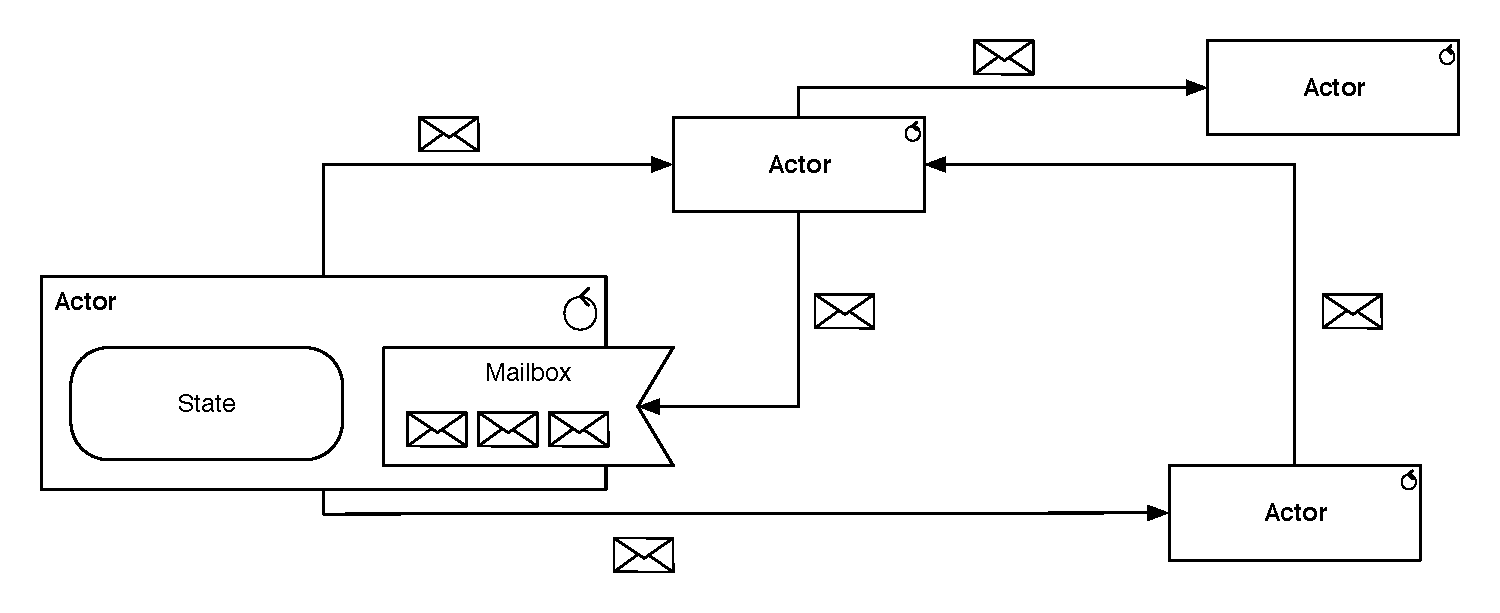
\includegraphics[width=1.0\textwidth]{4-Hauptteil/actor-model/actor-model.eps}
 \caption{Graphisches Beispiel einer Actor-basierten Anwendung.}
 \label{fig:actor-model}
\end{figure}

Ein Actor ist die kleinste Einheit in einer Actor-basierten Anwendung im Sinne des \enquote{Single Responsibility Principle} (siehe \textbf{??}), wie das graphische Beispiel eines Bestellvorgangs (\ref{fig:actor-model}) zeigen soll~\cite[S.~13]{vernon_reactive_2016}.\\
Jeder Actor besitzt eine sogenannte Mailbox, diese dient als Zwischenspeicher für eingehende Nachrichten. Außerdem hat jeder Actor einen Namen bzw. eine Adresse. Um einem Actor eine Nachricht zu schicken, wird die Adresse des Actors benötigt. Die Adresse ermöglicht es, mit einem Actor über eine abstrakte Referenz zu interagieren und dies wiederum ermöglicht \textit{location transparency}. Die Übertragung einer Nachricht an die Mailbox ist von unbestimmter Dauer und erfolgt asynchron. Zudem wird keine Reihenfolge der eingetroffenen Nachrichten garantiert \cite[S.~84]{erb_concurrent_2012} \cite[S.~83]{kuhn_reactive_2015}.\\
Ein Actor arbeitet jede Nachricht aus der Mailbox sequenziell ab. Deshalb muss während der Verarbeitung nicht auf Probleme bzgl. Nebenläufigkeit geachtet werden~\cite[S.~14]{vernon_reactive_2016}.\\
Ein Actor kann auf drei verschiedene Weisen auf eine Nachricht reagieren \cite[S.~84]{erb_concurrent_2012}:

\begin{enumerate}
\item Ein Actor kann eine begrenzte Anzahl von Nachrichten an andere Actors schicken.
\item Ein Actor kann eine begrenzte Anzahl weiterer Actors erzeugen.
\item Ein Actor kann den eigenen internen Zustand ändern.
\end{enumerate}

Der Zustand eines Actors ist isoliert und kann nur von dem Actor selbst verändert werden. Zustandsänderungen und daraus resultierende Verhaltensänderungen wirken sich aufgrund der sequenziellen Abarbeitung erst auf nachfolgende Nachrichten aus. Aufgrund dieser Voraussetzung kann man mit einen Actor problemlos endliche Automaten implementieren \cite[S.~14]{vernon_reactive_2016} \cite[S.~84]{kuhn_reactive_2015}.\\
Actor-basierte Anwendungen setzen somit auf \textit{mutable state} --- jedoch wird dieser nicht geteilt. Ein Actor kapselt seinen Zustand und interagiert nur über Nachrichten mit anderen Actors (siehe \fullref{subsec:sharenothing}). Der isolierte Zustand und die sequenzielle Verarbeitung der Nachrichten ermöglichen außerdem die sogenannte \enquote{lock-free concurrency} innerhalb eines Actors \cite[S.~85]{kuhn_reactive_2015}.\\
Eine Actor-basierte Anwendung besteht aus vielen Actors. Zudem entsteht durch die o.g. zweite Eigenschaft, weitere Actors zu erzeugen, eine Actor Hierachie. Komplexe Prozesse werden aufgebrochen und jeder Actor ist für eine kleine Aufgabe bzw. einen Task im System zuständig.\\
Die Hierarchie ermöglicht es, dass Konzept der \textit{supervision} umzusetzen. Übergeordnete Actors sind für Koordination und Verteilung der Tasks via Nachrichten verantwortlich. Tasks werden an untergeordnete Actors delegiert. Zudem übernehmen übergeordnete Actors eine Kontrollfunktion. Verhält sich ein untergeordneter Actor fehlerhaft, werden Maßnahmen, wie beispielsweise ein Neustart des fehlerhaften Actors, ergriffen. Ein Actor kann Fehler seiner untergeordneten Actors auch weiter nach oben propagieren, um dem System die Möglichkeit zu geben, Fehler zu beheben~\cite[S.~15]{vernon_reactive_2016} \cite[S.~83]{kuhn_reactive_2015} \cite[S.~86]{erb_concurrent_2012}.\\

Das Actor Modell wurde poplär durch die Programmiersprache Erlang\footnote{https://www.erlang.org/} und das Framework Akka\footnote{http://akka.io}. Diese Actor Systeme abstrahiert die Koordination der parallelen Ausführung. Die Verarbeitung einer Nachricht innerhalb eines Actors erfolgt immer durch einen Thread. Während dieser Verarbeitung ist ein Thread ausschließlich für einen spezifischen Actor zuständig.\\
Die Erlang VM startet beispielsweise einen Thread pool mit so vielen Threads, wie Rechenkerne zur Verfügung stehen. Diese Threads werden nun Actors zugewiesen, deren Mailboxen Nachrichten enthalten. Aufgrund der limitierten Ressourcen darf ein Actor einen Thread nicht für immer blockieren. Ähnlich, wie bei der ereignisbasierter Concurrency (\ref{subsec:eventdriven-concurrency}), ist deshalb \textit{Asynchronous I/O} für das Actor Modell vorteilhaft. Durch Scheduling, wie man es auch von Betriebsystemen kennt, achtet das Actor System auf Fairness, um \textit{starvation} einzeler Actors zu verhindern.\\

Mit einer Actor-basierten Anwendung ist es möglich eine Anwendung message-driven zu entwickeln. Beide Implementierungen, sowohl Erlang als auch Akka unterstützen die Verteilung von Actors auf mehrere Nodes und vorallem die Kommunikation via Nachrichten über mehrere Nodes hinweg. Somit skalieren Actor-basierte Systeme horizontal und vertikal. Bezüglich \textit{resilience} bietet die Actor Hierachie und das Konzept der \textit{supervision} eine gute Basis, um eine Anwendung von vornherein \textit{resilient} zu entwerfen.\\

Beide Concurrency Modelle bieten je nach Implementierung essentielle Konzepte, um reaktive Anwendung zu entwickeln.

\pagebreak

\section{Reaktive Programmierung}
Reaktive Programmierung, im weiteren Sinne, ist in der Entwicklung von Benutzeroberflächen üblich und verbreitet. Eine Software mit Benutzernutzeroberfläche muss stetig auf Eingaben durch den Benutzer reagieren. Dazu gehören neben Tastatureingaben und Mausklicks auch Cursorbewegungen. Dieser stetige Strom von neuen Informationen und Ereignissen muss verarbeitet werden, ohne dabei die Benutzeroberfläche zu blockieren. Nichts ist ärgerlicher, als eine Software, die nach einem Klick auf einen Button nicht reagiert bis der Vorgang abgeschlossen ist. Ebenso verhält sich es mit Serveranwendungen, die auf eine Vielzahl von gleichzeitigen Anfragen reagieren müssen.\\
Zu Beginn der Arbeit wurde bereits die Definition reaktiver Systeme von Harel und Pnueli genannt. Allgemeiner betrachtet bedeutet das englische Wort \textit{reactive} laut dem Merriam-Webster Wörterbuch \enquote{readily responsive to a stimulus}. Demnach ist etwas \textit{reactive}, wenn es bereitwillig auf einen Reiz reagiert. Im Bezug auf Software sind Reize beispielsweise Cursorbewegungen, Mausklicks oder Anfragen. Konkreter formuliert sind diese Reize Ereignisse, die von einer Komponente verarbeitet werden. Folgich ist ein Ereignis (engl. event) ein Signal über eine Zustandsänderung. Eine Komponente sendet ein Ereignis an seine Empfänger. Die reaktive Programmierung beschäftigt sich mit der nebenläufigen und asynchronen Verarbeitung dieser Ereignisse, um die \textit{responsiveness} der Anwendung sicherzustellen~\cite{rappl_introduction_2016}~\cite[S.~4]{carkci_dataflow_2014}~\cite[S.~5]{blackheath_functional_2015}.

\section{Observer-Pattern}
Ein Ereignis (engl. event) ist ein Signal bzw. ein Fakt über eine Zustandsänderung. Eine Komponente emittiert bzw. veröffentlicht ein Ereignis an seine Empfänger bzw. Beobachter. Hierfür nutzt man traditionellerweise das Verhaltensmuster \textit{observer}. Ein Beobachter (engl. observer) hat die Möglichkeit sich für Zustandsänderungen an- und abzumelden.\\
Folgendes Scala Codebeispiel zeigt das Observer-Pattern durch das Trait \textit{EventEmitter} (\ref{lst:lst5}). Beobachter, im Codebeispiel \textit{Observer} genannt, können sich über die Methoden \textit{subscribe} und \textit{unsubscribe} beim \textit{EventEmitter} an- und abmelden. Kommt es zu einer Zustandsänderung kann der \textit{EventEmitter} alle \textit{Observer} durch den Aufruf von \textit{emit} über das Ereignis informieren. Der \textit{EventEmitter} weiß nur, dass die \textit{Observer} die Methode \textit{handle} implementieren, die durch \textit{emit} aufgerufen wird.

\begin{lstlisting}[caption={Codebeispiel für das Observer-Pattern.},label={lst:lst5}]
trait EventEmitter {
  private var observers: Set[Observer] = Set()

  def subscribe(observer: Observer): Unit = observers += observer
  def unsubscribe(observer: Observer): Unit = observers -= observer
  def emit(): Unit = observers.foreach(_.handle(this))
}

trait Observer {
  def handle(emitter: EventEmitter): Unit
}
\end{lstlisting}

\pagebreak

\begin{lstlisting}[caption={Codebeispiel für das Observer-Pattern.},label={lst:lst6}]
class IncrementButton extends EventEmitter {
  private var counter = 0

  def getCount = counter
  def clicked(): Unit = {
    counter += 1
    emit()
  }
}

class IncrementLogger(button: IncrementButton) extends Observer {
  button.subscribe(this)

  def handle(emitter: EventEmitter): Unit = println(s"new value \${button.count}")
}

val button = new IncrementButton()
val logger = new IncrementLogger(button)

button.clicked() // prints: new value 1
button.clicked() // prints: new value 2
button.clicked() // prints: new value 3
button.clicked() // prints: new value 4
\end{lstlisting}

\subsection{Observables}
%TODO Reactive extensions & Observable 
%TODO Deprecating the Observer Pattern
%TODO Erik Meijer Talk about What is reactive?
%TODO Lesli Lamport We should use mathematics!
%TODO Rx are libraries for asynchronous and therefore reactive programming.

\pagebreak

\section{Reactive Design Patterns}
\subsection{Single Responsibility Pattern}
\subsection{Idempotent Receiver}
\subsection{Reactive Streams}
\subsection{Circuit Breaker}
% Enterprise Integration Patterns: Message, Message Channel, Event Message, Event-Driven Consumer
